\section{Zadání}

Analyzujte např. šance studenta na přijetí na VŠ, kdy jsou k dispozici „vhodná“ data:
\begin{itemize}
    \item ADMIT – binární informace o tom, zda student byl přijat na VŠ,
    \item GRE (Graduate Record Exam scores) – výsledky závěrečného hodnocení na SŠ,
    \item TOPNOTCH – binární informace o tom, zda absolvovaná SŠ patří mezi „top“ střední školy,
    \item GPA (Grade Point Average) – průměrné hodnocení na SŠ.
\end{itemize}

Sestavte a dokumentaci popište model charakterizující šance studenta na přijetí (pravděpodobnost) na VŠ a odhadněte parametry modelu.
Parametry odhadněte několika přístupy: pomocí probitů, logitů, MNČ a doporučte model na základě vybraného kritéria kvality (např. reziduální součet čtverců).
Upravte data (např. přidáním či odebráním, nebo změnou) ze souboru \textit{data04\_01.txt} nebo je možné též zvolit vlastní binární model a vlastní data.

\section{Data}

Pro vypracování semestrální práce nebyl zvolen avizovaný dataset o přijetí studentů, nýbrž dataset použitý již v minulé práci, tedy data o prodeji Monetových obrazů.
Tento dataset obsahuje 430 pozorování a 6 příznaků.
Příznaky jsou binární příznak značící zda-li je dílo podepsáno (vysvětlovaná proměnná), výška a šířka díla, cena [miliony USD] a kód aukčního domu, kde proběhla dražba (vysvětlující proměnné).

\section{Vypracování}

Pro zajímavější výsledky jsem výšku a šířku vynásobil, čímž jsem získal plochu obrazu a prohlásil ji za novou proměnnou.
V této semestrální práci budeme tedy predikovat, zda-li je prodaný Monetův obraz podepsaný, či nikoliv, z prodejní ceny, plochy obrazu a kódu aukčního domu.

Po rychlém nahlédnutí na data zjistíme, že obsahují nerovnoměrné zastoupení vysvětlované proměnné (353 podepsaných a 77 nepodepsaných děl).
Mějme na paměti, že takto biasovaná data budou (alespoň se tak domnívám) vychylovat výsledky ve prospěch toho, že dílo je podepsané.

Obrázek~\ref{fig:lr1} obsahuje vykreslené vysvětlující ku vysvětlované proměnné.

\begin{figure}[htb]
    \centering
    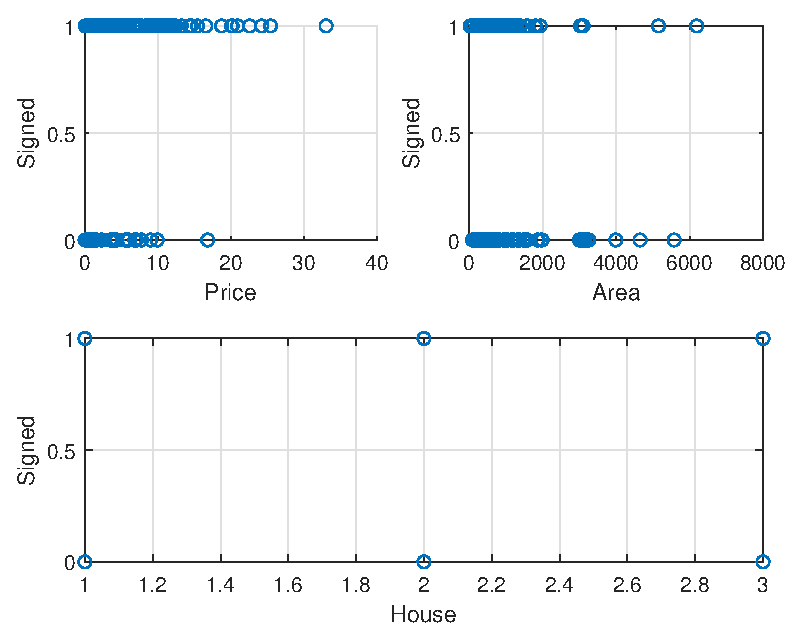
\includegraphics[width=0.7\textwidth]{graphs/fig1.eps}
    \caption{Vysvětlující ku vysvětlované proměnné}
    \label{fig:lr1}
\end{figure}
\FloatBarrier

Nejprve složíme matici příznaků (X), zavedeme lineární regresní model a otestujeme jeho vhodnost pomocí F-testu.
Po jeho vyhodnocení získáváme pro náš konkrétní model p-hodnotu rovnu \( 4.6336 \times 10^{-11} \).
Výsledek je menší než hladina \( \alpha = 5 \: \% \), zamítám tedy \( H_0 \) (všechny koeficienty \( \beta \) jsou rovny nule), a přijímám \( H_A \) (alespoň jeden koeficien je různý od nuly).
Zvolený model má tedy smysl a můžeme pokračovat dále.

Otestujeme vhodnost jednotlivých koeficientů \( \beta_i \) t-testem a získáváme následující p-hodnoty.

\begin{equation*}
    1.0 \times 10^{-3} \cdot \left[ \begin{matrix} 0.0000 \\ 0.0021 \\ 0.0000 \\ 0.5348 \end{matrix} \right]
\end{equation*}

Vektor p-hodnot pro každý z koeficientů modelu,

Hodnoty vyšší než \( \alpha = 5 \: \% \) vedou k zamítnutí \( H_0 \) (koeficient je rovný nule) a značí statistickou insignifikanci daného parametru.
V tomto případě kritérium nesplňuje žádný z parametrů, tudíž není třeba žádnou vysvětlující proměnnou z modelu vyřadit.

Podívejme se, jak budou vypadat modely odhadnuté pomocí \textit{logit}, \textit{probit} a \textit{metodou nejmenších čtverců} při vykreslení \( y \) vůči \( x_i \).
První obrázek dává do souvislosti podpis autora s prodejní cenou obrazu.
Ihned si můžeme povšimnout jevu, který je pravděpodobně způsoben rozdělením dat.
I při nejnižší prodejní ceně je dle tohoto příznaku téměř \( 80 \: \% \) pravděpodobnost, že je obraz podepsaný.

\begin{figure}[htb]
    \centering
    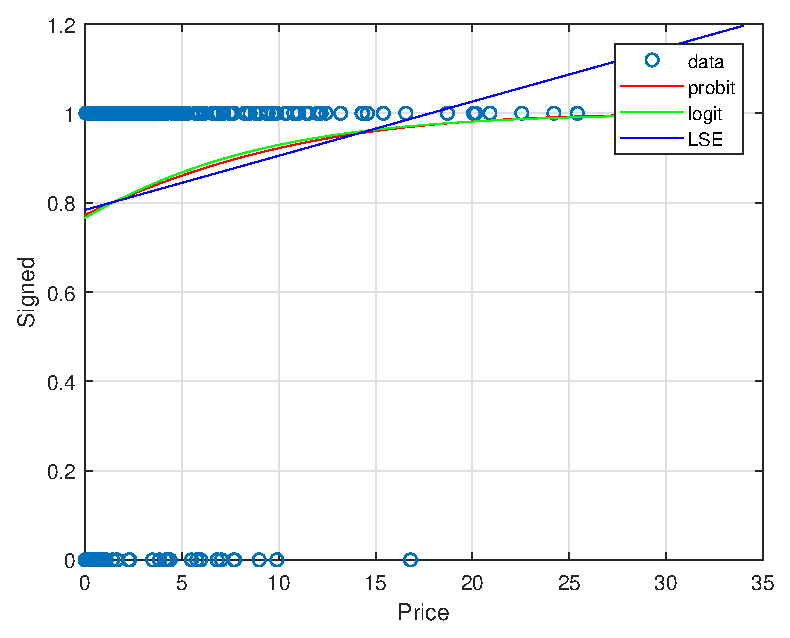
\includegraphics[width=0.55\textwidth]{graphs/fig2.eps}
    \caption{Srovnání modelů pro \( y \) vůči \( x_1 \)}
    \label{fig:lr2}
\end{figure}
\FloatBarrier

Podívejme se tedy na další graf, který dává do souvislosti podpis s plochou díla.
Tento graf je zajímavý, protože regresní křivky jsou vykreslené téměř celé a pokrývají značnou část pravděpodobnostního prostoru.

\begin{figure}[htb]
    \centering
    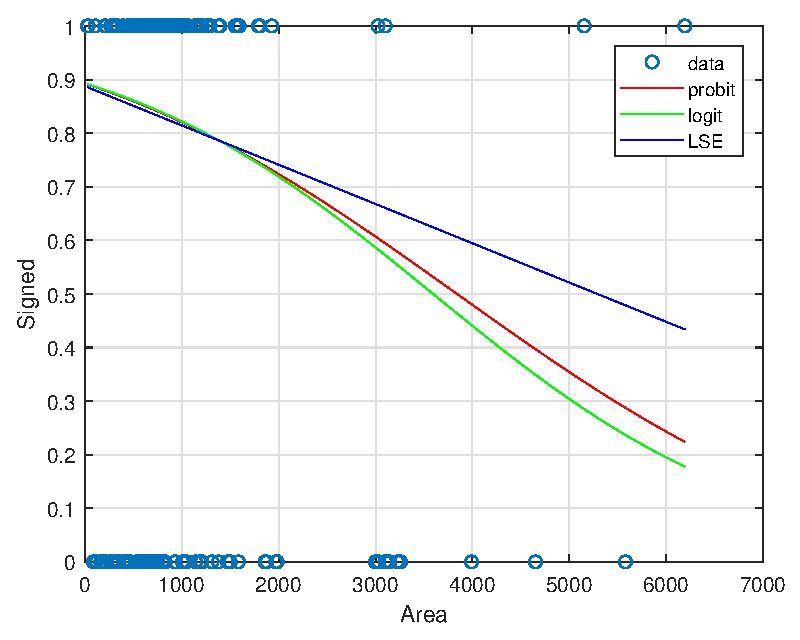
\includegraphics[width=0.55\textwidth]{graphs/fig3.eps}
    \caption{Srovnání modelů pro \( y \) vůči \( x_2 \)}
    \label{fig:lr3}
\end{figure}
\FloatBarrier

Na posledním grafu je patrný datový bias a pouze z grafu by bylo velice nepatřičné dělat jakékoliv závěry.

\begin{figure}[htb]
    \centering
    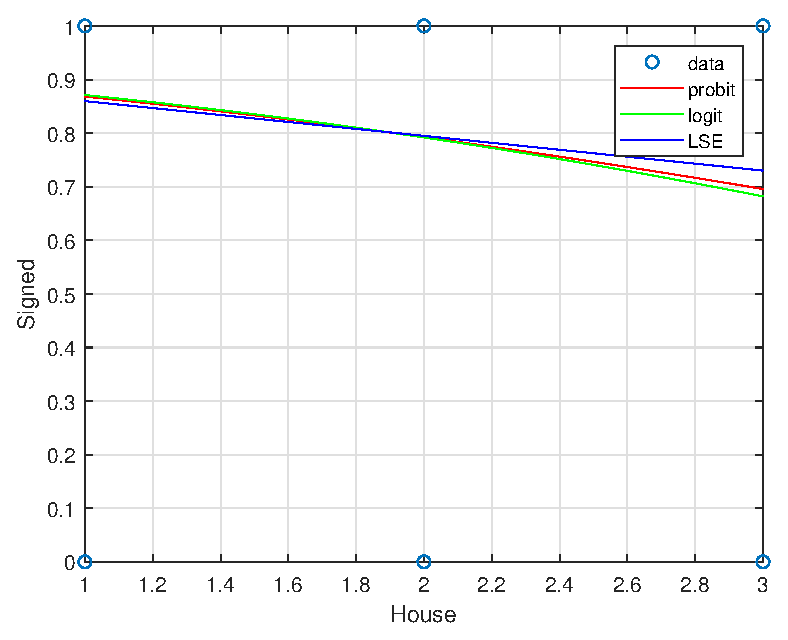
\includegraphics[width=0.55\textwidth]{graphs/fig4.eps}
    \caption{Srovnání modelů pro \( y \) vůči \( x_3 \)}
    \label{fig:lr4}
\end{figure}
\FloatBarrier

Konečnou vhodnost modelu získáme porovnáním nějaké metriky, např. \textit{rezidálního součtu čtverců} jednotlivých modelů.
Po sestavení modelů z celé matice příznaků \( X \) a vypsání reziduálního součtu pro každý z modelů získáváme následující hodnoty.

\begin{table}[htb]
    \centering

    \begin{tabular}{lll}
        \toprule

        Metoda  & Rezidální součet čtverců  \\ \midrule
        Probit  & 346.3584                  \\
        Logit   & 344.4648                  \\
        MNČ     & 458.2582                  \\
          
        \bottomrule
    \end{tabular}

    \caption{Rezidální součet čtverců}
    \label{table:table1}
\end{table}
\FloatBarrier

Z tabulky~\ref{table:table1} přečteme, že nejmenší hodnoty jsou u metod \textit{logit} \& \textit{probit}.
Jestliže by kritériem výběru nejlepší metody bylo minimum RSČ, pak bychom za nejlepší metodu označili \textit{logit}.

\section{Závěr}

V semestrální práci jsme si vyzkoušeli modelování binárního regresoru.
Pomocí vizualizací jsme získali představu o fungování představených metod.
Využití statistických testů nám zase upevnilo znalosti nutné pro volbu vhodných modelů a případné odstranění nevhodných proměnných.
